\subsection{Structure manipulation}
Let's explore changing the structure of the target matrix and the decomposition products. The results are interesting.
There are two basic matrix operations: shifts ($\Delta$) and flips ($\K{}$). When these operators are \emph{pre}multipliers they change the \emph{row} structure. When they \emph{post}multiply they change the \emph{column} structure.

%%%%%%%%%%%
%%%%%%%%%%%
\subsection{Shifts}
Consider the example of shifting $s=40$ places. The first instance pushes the rows down; the second instance pushes the columns to the right:
\begin{equation}
  \begin{split}
    %
    \Delta(40) \, \A{} &= \mat{ccc}{
    a_{41,1} &  \dots & a_{41,n} \\
      \downarrow && \downarrow \\
    a_{m,1}  &  \dots & a_{m,n} \\\hline
    a_{1,1} &  \dots & a_{1,n} \\
      \downarrow && \downarrow \\
    a_{40,1}  &  \dots & a_{40,n}
    }, \\[10pt]
    %
    \A{} \, \Delta(40) &= \mat{ccc|ccc}{
    a_{1,41} &  \rightarrow & a_{1,n} & a_{1,1} &  \rightarrow & a_{1,40} \\
      \vdots && \vdots & \vdots && \vdots \\
    a_{m,41} &  \rightarrow & a_{m,n} & a_{m,1} &  \rightarrow & a_{m,40} \\
    }.
    %
  \end{split}
\end{equation}
We see that when $\Delta(40)$ acts on the \emph{left} (\emph{pre}multiplication) the result is that row 41 becomes the first row. When $\Delta(40)$ acts on the \emph{right} (\emph{post}multiplication) the result is that column 41 becomes the first column. The general case follows.

As usual, let the target matrix $\A{}$ have $m$ rows and $n$ columns. To push the columns $s$ places to the right use the $\byy{m}$ matrix
\begin{equation}
  \Delta_{m}(s) = \mat{c|c}{
  \zero_{1} & \I{m-s} \\\hline
  \I{s}     & \zero_{2}
  } .
\end{equation}
One should verify that $\zero_{1}$ has dimension $\byy{ \paren{m-s} }$ and that $\zero_{2}$ has dimension $\by{ s }{m - s}$. To push the rows $s$ places down use the $\byy{n}$ matrix
\begin{equation}
  \Delta_{n}(s) = \mat{c|c}{
  \zero_{3} & \I{n-s} \\\hline
  \I{s}     & \zero_{4}
  } .
\end{equation}
The matrix $\zero_{3}$ has dimension $\byy{ \paren{n-s} }$; $\zero_{4}$ has dimension $\by{ s }{n - s}$.

This is a representative shift
\begin{equation}
  \Delta_{m}\paren{200} \A{} =
  \raisebox{-0.5\height}{\includegraphics[ width = 1.22in ]{images/"information content I"/structure/"shift 200"}}
  \raisebox{-0.5\height}{\includegraphics[ width = 1in ]{images/"information content I"/structure/"camille"}} =
  \raisebox{-0.5\height}{\includegraphics[ width = 1in ]{images/"information content I"/structure/"naked shift"}}
\end{equation}
%

%%%%%%%%%%%
%%%%%%%%%%%
\subsection{Flips}
The flip matrix $\K{}$ is constructed by reordering the column vectors of an identity matrix. We can flip an image vertically (right-left) and we can flip an image horizontally (up-down). 
Given a target matrix $\A{}$ with $m$ rows and $n$ columns, the matrix which flips the \emph{columns} is constructed using the column vectors from the identity matrix $\I{m}$:
\begin{equation}
  \K{m} = \mat{ccc}{e_{m} & \dots & e_{1}}.
\end{equation}
Similarly, the matrix which flips the \emph{rows} is constructed using the column vectors from the identity matrix $\I{n}$.
The operations are:
\begin{equation}
  \begin{split}
    %
    \A{} \, \K{n} &= \mat{ccc}{
    a_{1,n} &  \leftarrow & a_{1,1} \\
     \vdots && \vdots \\
    a_{m,n} &  \leftarrow & a_{m,1}
    }, \\[10pt]
    %
    \K{m} \A{} &= \mat{ccc}{
    a_{m,1} &  \dots & a_{m,n} \\
    \uparrow && \uparrow \\
    a_{1,1}  &  \dots & a_{1,n}
    }.
    %
  \end{split}
\end{equation}
This is a representative column flip
\begin{equation}
  \A{} \K{n} =
  \raisebox{-0.5\height}{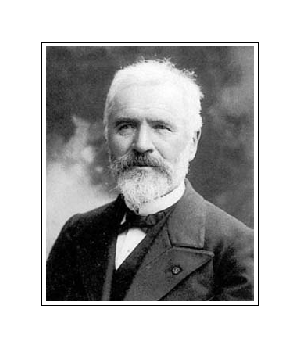
\includegraphics[ width = 1in ]{images/"information content I"/structure/camille}}
  \raisebox{-0.325\height}{\includegraphics[ width = 0.816in ]{images/"information content I"/structure/"flip cols"}} =
  \raisebox{-0.5\height}{\includegraphics[ width = 1in ]{images/"information content I"/structure/"flipped cols"}}
\end{equation}
%
%%%%%%
\input{chapters/"information content I"/"tab matrix structure manipulation flip"}   % table
\input{chapters/"information content I"/"tab matrix structure manipulation shift"}  % table

%%%%%%%%%%%
%%%%%%%%%%%
\subsection{Compositions of structure operations}
The flip matrix is involutary:
\begin{equation}
  \K{m} \K{m} = \I{m}
\end{equation}
An improper reflection.

The shift matrix
\begin{equation}
  \Delta_{m}\paren{j}\Delta_{m}\paren{k} = \Delta_{m}\paren{j+k}
\end{equation}
As one may expect, 
%
\begin{equation}
  \Delta_{m}\paren{j} \Delta_{m}\paren{k} = \Delta_{m}\paren{j+k}
\end{equation}
%
\begin{table}[htdp]
\caption{The shift matrices are additive in the shift index}
\begin{center}
\begin{tabular}{cccc}
%
  $\Delta_{m}\paren{200}$ & $\Delta_{m}\paren{80}$ &=& $\Delta_{m}\paren{280}$ \\
%
  \includegraphics[ width = 1in ]{images/"information content I"/structure/"shift 200"} &
  \includegraphics[ width = 1in ]{images/"information content I"/structure/"shift 80"} &&
  \includegraphics[ width = 1in ]{images/"information content I"/structure/"shift 280"}
%
\end{tabular}
\end{center}
\label{tab:structure:shifts add}
\end{table}%

\begin{equation}
  \K{m}\, \Delta_{m}\!\paren{250} \A{}\, \Delta_{n}\!\paren{80}\, \K{n} =
  \raisebox{-0.5\height}{\includegraphics[ width = 1.5in ]{images/"information content I"/structure/"composite"}}
\end{equation}

%%%%%%%%%%%
\subsection{Structure manipulation and the SVD}
How does the SVD change under these structure manipulations?
\begin{equation}
  \begin{split}
    \Delta_{m}\!\paren{j} \A{}  &= \Delta_{m} \svd{*} = \paren{\Delta_{m}\!\paren{j} \U{}} \sig{} \, \V{*} = \tilde{\U{}} \sig{} \, \V{*}\\
    \A{}\, \Delta_{n}\!\paren{k}  &= \svd{*}\Delta_{n}\!\paren{k} = \U{} \, \sig{} \, \paren{\V{*}\Delta_{n}\!\paren{k}} = \U{} \, \sig{} \, \tilde{\V{*}}
  \end{split}
\end{equation}
The unitary matrices absorb the transformation.


\endinput